\section{Standard Model}
The Standard Model (SM) is the leading theory that describes interactions between particles at a subatomic scale. I begin with a brief summary of the SM itself beginning with brief descriptions of the fundamental particles and their forces before delving into a summarized mathematical formulation. Next, I discuss the history of the SM and crucial tests of the theory up until current work at the LHC.  I will then  outline some of the recent and current physics at the Large Hadron Collider (LHC) with a focus on Higgs boson measurements. Finally, I'll introduce my thesis' main focus, differential cross-section measurements of Vector-Boson-Fusion Higgs decaying into two W-bosons.

The Standard Model is one of the most successful scientific theories to date. Its predictions encompass all of the visible universe and continue to undergo careful testing. The SM combines three forces- electromagnetic, weak, and strong - into one elegant description. I'll follow in the steps of many before me and detail the theory through first introducing particles and forces. Next I will introduce the mathematical formalisms describing particle interactions.
\subsection{Particles and forces}
 The particles we define in high energy physics are the most minute portions of matter we're able to observe. They are generally considered point-like, have no internal structure, and cannot be further split. Each particle we can define has a unique set of quantum numbers and its own anti-particle (with the same mass and spin, but opposite electrical charge and quantum numbers).

Particles can split up into distinct groups- first bosons, with integer spin, and fermions, with half-integer spin. Bosons are 'force carriers' meaning when particles interact they exchange bosons. Fermions are at the heart of all conventional matter. Fermions can be split further into two categories- leptons and quarks. Quarks have fractional integer charge and interact strongly while leptons have integer charge and interact solely through the weak or electromagnetic forces. Both quarks and leptons are made of three generations of particles, each heavier and more unstable than the next. Charts showing quark/lepton families and their key quantum numbers are shown below. Each generation of quarks and leptons contains a particle doublet. Each lepton doublet contains a charged lepton and a neutrino while each quark doublet contains one $+2/3$ charged particle and one with a $-1/3$ charge. Each lepton and quark also has an anti-particle. All conventional, stable matter is made from the first generation of quarks and leptons.

There are four gauge bosons and one scalar boson predicted through the SM. These correspond to three fundamental forces in nature (the fourth, gravity, is so small on the scale of particle interactions as to not be considered). The strongest force on the subatomic scale is the strong force- this is mediated by the gluon- and works primarly to bind quarks together to form composite particles like protons or neutrons. The electromagnetic force is about 60x weaker than the strong force and is mediated by the photon. This force accounts for all electric interactions like that between an electron an an atomic nucleus. Finally, the weak force ($10^4$ weaker than the EM) facilitates $\beta$-decay and is mediated by massive Z and W bosons. Before going into more detail on the gauge bosons and the forces they mediate, I'd be remiss not to mention the Higgs boson. The only scalar boson predicted by the SM, it is has no charge or intrinsic spin. The Higgs gives mass to all other particles through Spontaneous Symmetry Breaking, which I'll expand on in later sections.
\begin{figure}[H]
	\centering
    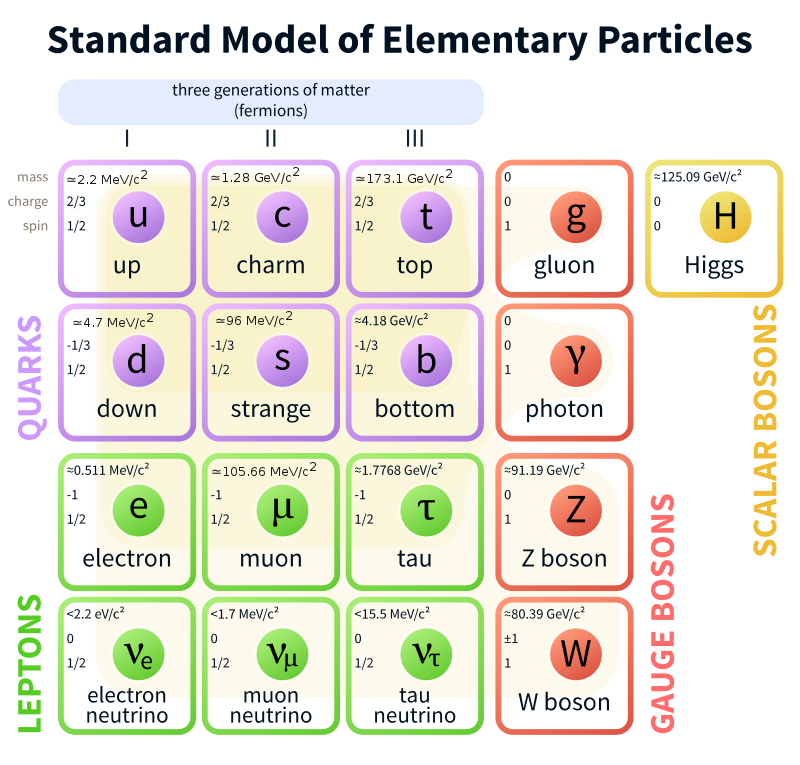
\includegraphics[width=0.7\textwidth] {Pictures/SMparticles.png}\hspace{1cm}
    \caption{Three generations of quarks and leptons are shown along with all SM bosons \cite{PDG}}
    \label{fig:SMparticles}
\end{figure}
Photons are massless, spin-1 particles and mediate all electromagnetic interactions. They couple directly to any particle with electric charge- so quarks, leptons, and $W$/$Z$ bosons but not neutrinos. Since the photon is massless, the electromagnetic force can operate on infinitely long scales but it's force decreases with $1/r^2.$
 
Gluons are massless particles with no charge and a spin-1. They couple to color charges, which are a property of quarks. Each quark has one of three colors (RGB) while anti-quarks have "anti" versions of these. Colors ore conserved 'charges' just like electric charge. Quarks are never found alone as they couple so strongly to one another as to be confined in groups of two or three. These groups are "color-confined" meaning the quarks contain colors which add up to a color neutral sum. For instance, a two quark meson $u\bar{u}$ may have colors R and anti-R while a three quark hadron $uud$ (proton) may have colors R, G, and B. Gluons are different from photons in that they are not neutral to the charge they couple to. Gluons have two colors (8 total combinations) and can thus couple to each other. This makes the strong force distinct from the electromagnetic and has implications for long-distance interactions.
 
$W$ and $Z$ bosons, unlike gluons and photons, are massive. However, like their other gauge boson counterparts, they have spin-1 and mediate a charge (weak). $W^{\pm}$ mediates charged-current interactions which can violate flavor conservation between quarks and/or leptons and their neutrinos. $Z^{0}$ mediates neutral-current interactions which conserve flavor. $W^{\pm}$ bosons contain electric charge so can interact through EM as well. In addition, $W$ and $Z$ bosons contain weak charge (as do all fermions) so can self-couple as well as couple with all fermions. 
 
The Higgs boson will be further motivated and described in later sections but suffice to say it's a massive spin-0 particle which couples to all particles with mass (including itself). It doesn't mediate any force but is still an integral part of the SM.  

\subsection{Gauge Invariance}
According to Noether's theorem, for every continuous transformation of a field that leaves the Lagrangian invariant, there is a conserved current. Symmetries found in physical theories lead to conservation laws (and vice-versa). The Standard Model is a gauge theory built on symmetries such that all interactions between particles result from requiring the theory to be invariant under local gauge transformations. Each part of the Standard Model- from quantum electrodynamics (QED) to quantum chromodynamics (QCD) - is a gauge theory on its own, which simply means they have gauge invariance symmetries. In this section I'll step through the basic mathematic formalism for QED, QCD, and the combined electro-weak theory to illustrate the physical ramifications of gauge invariance and set the stage for the Higgs mechanism. The following sections are written with guidance from text \cite{HalzenMartin}. 

\subsubsection{Quantum Electrodynamics}
Quantum electrodynamics (QED) is the first, and simplest, physical gauge theory, describing how light and matter interact even under relativistic conditions. The theory produces extremely good agreement with experiment due to the success of perturbative solutions and entire textbooks are dedicated to its motivation and calculated predictions. Here I will generate the full QED Lagrangian by imposing local gauge invariance on the Lagrangian of a free fermion. 

First, the Dirac Lagrangian describes a free fermion of mass \textit{m}
\begin{equation}
\mathcal{L} = i \psi \gamma^\mu \partial_ \mu \psi - m\bar{\psi}\psi,
\end{equation}
where $\psi$ is a Dirac spinor and $\gamma^\mu$ represent the Dirac matrices. To demonstrate local gauge invariance we need to transform
\begin{equation}
\psi(x) \rightarrow e^{i\alpha(x)}\psi(x) 
\end{equation}
where $\alpha(x)$ depends on space and time arbitrarily. Directly substituting this into our Lagrangian shows that $\mathcal{L}$ is not invariant, and the $\partial_\mu$ term breaks this
\begin{equation}
\partial_\mu \psi \rightarrow e^{i\alpha(x)}\partial_\mu\psi + ie^{i\alpha(x)}\partial_\mu \alpha
\end{equation}
In order to mandate the theory is invariant we need to change this term to the "covariant derivative" $D_\mu$ which transforms 
\begin{equation}
D_\mu\psi \rightarrow e^{i\alpha(x)}D_\mu\psi . 
\end{equation}	 
In order to transform as such the "covariant derviative" has to contain a vector field $A_\mu$ and this field must transform so as to cancel with the unwanted part of the transformed $D_\mu$. 
\begin{equation}
D_\mu \equiv \partial_\mu - ieA_\mu
\end{equation}
where 
\begin{equation}
A_\mu \rightarrow A_\mu + \frac{1}{e}\partial_\mu \alpha
\end{equation}
Now the original Dirac equation is replaced with the following:
\begin{equation}
\mathcal{L} = \bar{\psi}(i\gamma^\mu\partial_\mu-m)\psi + e\bar{\psi}\gamma^\mu\psi A_\mu.
\end{equation}
By requiring local gauge invariance we've introduced a gauge field $A_\mu$ which couples to the Dirac particle just as the photon. In fact, if we take this as the photon gauge field and so add a kinetic energy term (which is also local gauge invariant!) we find the Lagrangian of QED. 
\begin{equation}
\mathcal{L} = \bar{\psi}(i\gamma^\mu\partial_\mu-m)\psi + e\bar{\psi}\gamma^\mu\psi A_\mu -\frac{1}{4} F_{\mu\nu}F^{\mu\nu}
\end{equation}
One can also see that adding a mass term to the Lagrangian for the new field ($\frac{1}{2}m^2A_\mu A^\mu$) would break gauge invariance, indicating the photon must be massless. From the free fermion Lagrangian, imposing local gauge invariance leads to the full interacting field theory of QED. This isn't a curiosity but an essential component of the theory, and the use of local gauge symmetry in deriving particle interactions doesn't end here.
\subsubsection{Quantum chromodynamics}
Quantum chromodynamics differs from QED in a few crucial ways. First, since quark color fields exist the QED $U$(1) gauge group is replaced with $SU$(3) and the free Lagrangian contains indices $j$ to denote the three color fields. 
\begin{equation}
\mathcal{L} = \bar{q}_j(i\gamma^\mu\partial_\mu - m)q_j.
\end{equation}
QCD also carries three quark flavors, which will be ignored here for simplicity. The QCD group is also non-Abelian since not all generators of the group commute with each other. These generators will be defined as $T_a$ where $=1,...,8$ and are linearly independent traceless $3\times3$ matrices (the Gell-Mann matrices $\lambda_a$ are conventional). The local color phase transformation required is thus 
\begin{equation}
q(x) \rightarrow e^{i\alpha_a(x)T_a}q(x)
\end{equation}
We can consider an infinitesimal phase transformation as 
\begin{equation}
q(x) \rightarrow [1+i\alpha_a(x)T_a]q(x), \\
\partial_uq \rightarrow (1+i\alpha_aT_a)\partial_\mu q + i T_a q \partial_\mu \alpha_a.
\end{equation}
Just as in the QED example, the last line breaks the invariance of $\mathcal{L}$ and we can proceed very similarly to the QED case by introducing a new gauge field (or in this case eight) called $G_\mu^a$ which transform 
\begin{equation}
G_\mu^a \rightarrow G_\mu^a - \frac{1}{g}\partial_\mu\alpha_a - f_{abc}\alpha_b G_\mu^c
\end{equation}
The last term added here is to cope with the non-Abelian nature of QCD (that not all the generators $T_a$ commute with each other). Just as in QED this invariance forms a covariant derviative 
\begin{equation}
D_\mu = \partial_mu + i g T_aG_\mu^a
\end{equation}
Replacing the derivative into our Lagrangian and adding a gauge invariant energy term for each of the $G_mu^a$ fields ($\frac{1}{4}G_{\mu\nu}^aG_{\mu\nu}^a$) yields the final gauge invariant QCD Lagrangian
\begin{equation}
\mathcal{L} = \bar{q}(i\gamma^\mu\partial_\mu - m)q - g(\bar{q}\gamma^\mu T_aq)G_\mu^a-\frac{1}{4}G_{\mu\nu}^aG_{\mu\nu}^a.
\end{equation}
Just as in the QED case, imposing local color phase invariance produced a new interacting field (or rather, eight) with a coupling specified as $g$. These are the gluon fields and just like photons, local gauge invariance requires them to be massless. Unlike the QED case, this Lagrangian's new kinetic term includes self-interaction between the gauge bosons - another key feature of QCD that is mandated by local color phase invariance. Gluons themselves must carry color charge and so self-couple - the structure of these self coupling terms and their single coupling strength $g$ are uniqely determined by gauge invariance. 
\subsubsection{Electro-weak unification?}

\subsubsection{Spontaneous Symmetry Breaking}
Unlike QED and QCD, the weak force is mediated by massive gauge bosons. Because of this, we can't apply the same gauge invariance prescription that we did in the last sections. If a mass term is added to the Lagrangian we break the gauge invariance we aimed to find. If we instead ignore the gauge invariance and add a mass term to the Lagrangian, all predictive power of the theory is lost due to unrenormalizable divergences. With "spontaneous symmetry breaking" we can gain massive gauge bosons while maintaining the integrity of the theory. In this section I first describe the "spontaneous symmetry breaking" mechanism is terms of an Abelian theory composed of complex scalar fields to illustrate the overall strategy. This mechanism is then applied to the non-Abelian electroweak theory to gain massive weak gauge bosons $W^{+/-}$ and $Z$, with the Higgs field appearing as a 'spontaneous' result.

The Lagrangian for a $U$(1) gauge symmetry 
\begin{equation}
\phi \rightarrow e^{i\alpha(x)}\phi
\end{equation}
As in the QED case, we introduce a gauge field $A_\mu$ and covariant derivative $D_\mu = \partial_\mu - ieA_\mu$ to obtain the gauge invariant Lagrangian
\begin{equation}
\mathcal{L} = (\partial^\mu+ieA^\mu)\phi^*(\partial_mu-ieA_\mu)\phi-\mu^2\phi^*\phi-\lambda(\phi^*\phi)^2-\frac{1}{4}F_{\mu\nu}F^{\mu\nu}.
\end{equation}
In this example if $\mu^2>0$ we gain back the QED Lagrangian for a charged scalar particle of mass $\mu$ - with an additional self-interaction term. However, if we take $\mu^2<0$ the potential $V(\phi^*\phi)=\mu^2\phi^*\phi-\lambda(\phi^*\phi)^2$ now has a non-zero vacuum expectation value (v.e.v.) and there's a set of equivalent minima shown in Figure \ref{fig:HiggsPotential}. Choosing one of these minima spontaneously breaks the potential's rotational symmetry. Next, we can perturbatively expand the field about a minima through
\begin{figure}[H]
    \centering
    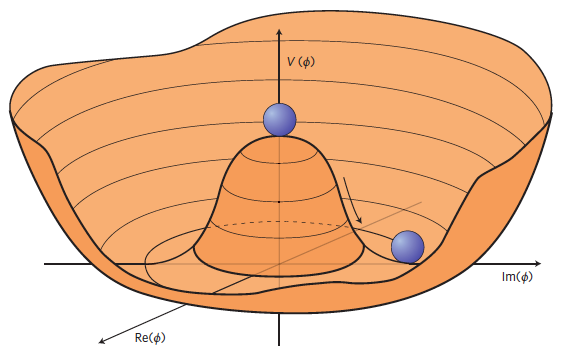
\includegraphics[width=0.5\textwidth] {Pictures/HiggsPotential.png}\hspace{1cm}
    \caption{Higgs potential when $\mu^2<0$, choosing a minima spontaneously breaks the $U$(1) rotational symmetry \cite{HiggsPotential}}.
    \label{fig:HiggsPotential}
\end{figure}

\begin{equation}
\phi(x) =\sqrt{\frac{1}{2}[\nu+\eta(x)+i\xi(x)]}
\end{equation}
Substituting this perturbation gives the new Lagrangian
\begin{equation}
\mathcal{L}'=\frac{1}{2}(\partial_\mu\xi)^2+\frac{1}{2}(\partial_\mu\eta)^2-\nu^2\lambda\eta^2+\frac{1}{2}e^2\nu^A_\mu A^\mu-e\nu A_\mu \partial^\mu\xi-\frac{1}{4}F_{mu\nu}F^{\mu\nu} + \textnormal{interaction terms}.
\end{equation}
Three particles seem to emerge here: massless Goldstone boson $\xi$, massive vector $A_\mu$ with $m_A=e\nu$ and a massive scalar $\eta$ with $m_\eta=sqrt{2\lambda\nu^2}$. However, the number of particles does not correspond to the polarization degrees of freedom expected, a longitudonal polarization was added, creating an unphysical field. To eliminate the unphysical field we can substitute new set of fields 
\begin{equation}
\phi \rightarrow \sqrt{\frac{1}{2}(\nu+h(x))e^{i\theta(x)/\nu}}
\end{equation}
and 
\begin{equation}
A_\mu \rightarrow A_\mu + \frac{1}{e\nu} \partial_\mu\theta.
\end{equation}
Introducing these substitutions, the Goldstone boson field disappears
\begin{equation}
\mathcal{L} = \frac{1}{2}(\partial_\mu h)^2 -\lambda\nu^2h^2+\frac{1}{2}e^2\nu^2A_\mu^2-\lambda\nu h^3-\frac{1}{4}\lambda h^4+\frac{1}{2}e^2A_\mu^2h^2+\nu e^2A_\mu^2h-\frac{1}{4}F_{\mu\nu}F^{\mu\nu}
\end{equation}
Here the degrees of freedom before our substitutions remains the same and a massive boson $A_\mu$ is preserved along with a massive scalar $h$. The "Higgs mechanism" applied to a scalar field succeeded in creating a massive boson and determined the existence of a Higgs boson. One can apply the same mechanism to the more complicated $SU$(2) gauge symmetry of electroweak interactions to determine the mass of the $W$ and $Z$ bosons and predict the existence of the Standard Model Higgs boson. 


\section{Brief history of SM tests}

\section{LHC Physics/Phenomenology}

\section{Measurement motivation}

